\begin{comment}


% \begin{figure}
%   \makebox[\textwidth][c]{
%   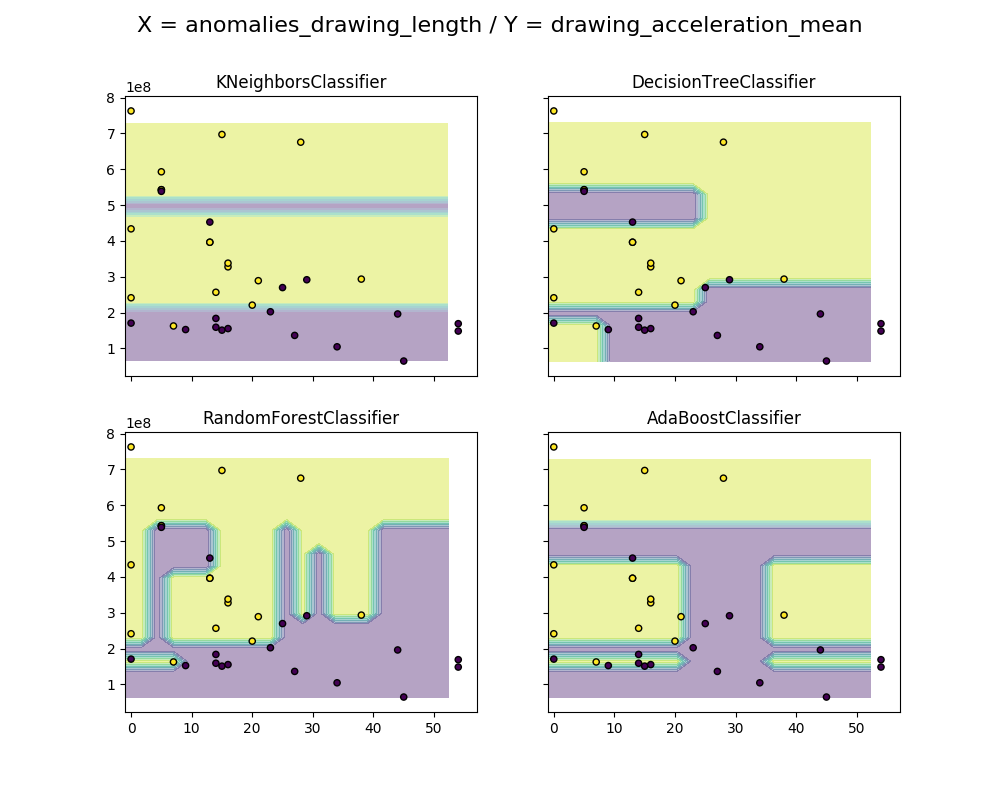
\includegraphics[width=1.7\textwidth]{images/classifier/001}}%
%   \caption{Caption}
%   \label{fig:key}
% \end{figure}


% Our aim was to build a discriminative model to differentiate between people with PD and HC. It is a binary classification task that can be resolved by statistical machine learning algorithms.

% The underlying idea of SVM classifiers is to calculate a maximal margin hyperplane separating two classes of the data. To learn non-linearly separable functions, the data are implicitly mapped to a higher dimensional space by means of a kernel function, where a separating hyperplane is found. New samples are classified according to the side of the hyperplane they belong to. 

% Decision Trees (DTs) are a non-parametric supervised learning method used for classification and regression. Decision trees learn from data to approximate a sine curve with a set of if-then-else decision rules. The deeper the tree, the more complex the decision rules and the fitter the model.

% Decision tree builds classification or regression models in the form of a tree structure. It breaks down a data set into smaller and smaller subsets while at the same time an associated decision tree is incrementally developed. The final result is a tree with decision nodes and leaf nodes. A decision node has two or more branches. Leaf node represents a classification or decision. The topmost decision node in a tree which corresponds to the best predictor called root node. Decision trees can handle both categorical and numerical data.

% each capable of producing a response when presented with a set of predictor values. For classification problems, this response takes the form of a class membership classifies, a set of independent predictor values with one of the categories present in the dependent variable.

% The essence of the technique is to construct multiple decision trees in randomly selected feature sub-space and use averaging to improve the predictive accuracy and control over-fitting. Using tree ensembles can lead to significant improvement in prediction accuracy (i.e., better ability to predict new data cases).

% Random forests or random decision forests are an ensemble learning method for classification, regression and other tasks, that operate by constructing a multitude of decision trees at training time and outputting the class that is the mode of the classes (classification) or mean prediction (regression) of the individual trees

% AdaBoost, short for Adaptive Boosting, is a machine learning meta-algorithm formulated by Yoav Freund and Robert Schapire, who won the 2003 Gödel Prize for their work. It can be used in conjunction with many other types of learning algorithms to improve performance. The output of the other learning algorithms ('weak learners') is combined into a weighted sum that represents the final output of the boosted classifier. AdaBoost is adaptive in the sense that subsequent weak learners are tweaked in favor of those instances misclassified by previous classifiers. AdaBoost is sensitive to noisy data and outliers. In some problems it can be less susceptible to the overfitting problem than other learning algorithms. The individual learners can be weak, but as long as the performance of each one is slightly better than random guessing, the final model can be proven to converge to a strong learner.

% AdaBoost is one of the important ensemble methods known as boosting. The key idea behind boosting techniques is to use ensemble methods to combine weak classifiers in order to build a strong learner. AdaBoost is an iterative boosting algorithm constructing a strong classifier as a linear combination of weak classifiers, each performing at least above chance level (50 correct classification). 

% We used decision trees classifiers as weak classifiers. The maximum number of estimators at which boosting is terminated was set to 500. Settings used for decision trees were as follows. The number of features to consider when looking for the best split was the square root of the number of features and the maximum depth of the tree was set to 3.

% Classifier validation was conducted using stratified 10-fold cross-validation. The data was divided into ten mutually exclusive and exhaustive equal-sized subsets. For each subset, the union of all other subsets was considered as training data and the error rate was determined. Errors over different subsets were averaged to obtain the classification error. The process was repeated a total of ten times; the original dataset was randomly permuted in each repetition prior to splitting into training and testing subsets. The results were averaged over all ten runs.
% The classification test performance was determined by the classification accuracy Pacc, sensitivity Psen and specificity Pspe.

% From all computed features we kept only those that passed the Mann–Whitney U test, i.e. those that showed a statistically significant (p < 0.05) difference between the PD and control groups. Table 3 shows 20 most relevant features and median of their values for PD and healthy control group. Features are sorted according Spearman’s correlation coefficient 
% The highest classification accuracy using pressure features Pacc = 74.2\% was obtained for data from the task 6

to apply 3-fold cross-validation, more specific This cross-validation object is a variation of KFold that returns stratified folds. The folds are made by preserving the percentage of samples for each class.

Stratified K-Folds cross-validator

Provides train/test indices to split data in train/test sets.
This cross-validation object is a variation of KFold that returns stratified folds. The folds are made by preserving the percentage of samples for each class.

StratifiedKFold implementation of $Scikit-learn$

% Classifier validation was conducted using stratified 10-fold cross-validation. The data was divided into ten mutually exclusive and exhaustive equal-sized subsets. For each subset, the union of all other subsets was considered as training data and the error rate was determined. Errors over different subsets were averaged to obtain the classification error. The process was repeated a total of ten times; the original dataset was randomly permuted in each repetition prior to splitting into training and testing subsets. The results were averaged over all ten runs.

% The classification test performance was determined by the classification accuracy Pacc, sensitivity Psen and specificity Pspe.
% From all computed features we kept only those that passed the Mann–Whitney U test, i.e. those that showed a statistically significant (p < 0.05) difference between the PD and control groups. Table 3 shows 20 most relevant features and median of their val- ues for PD and healthy control group. Features are sorted according Spearman’s correlation coefficient.

% % % % % % % % % % % % % % % % % % % % % % % % % % % % % % % % % % % %

% One round of cross-validation involves partitioning a sample of data into complementary subsets, performing the analysis on one subset (called the training set), and validating the analysis on the other subset (called the validation set or testing set). To reduce variability, in most methods multiple rounds of cross-validation are performed using different partitions, and the validation results are combined (e.g. averaged) over the rounds to estimate a final predictive model.

% One of the main reasons for using cross-validation instead of using the conventional validation (e.g. partitioning the data set into two sets of 70\% for training and 30% for test) is that there is not enough data available to partition it into separate training and test sets without losing significant modelling or testing capability. In these cases, a fair way to properly estimate model prediction performance is to use cross-validation as a powerful general technique.[5]



\end{comment}

\section{Methodology}

After previous analysis phase, statistically significant numeric feature subset was determined for labelled collection of drawings, received from Parkinson's disease patients PD and healthy control HC. Major goal of current research is to construct classifier model for HC and PD differentiation. Considering number of possible labels in dataset (PD and HC), we a dealing with standard \textit{binary classification} problem, which is solvable by machine learning algorithms. 

\subsection{Classifier Algorithms}

For the purpose of best performing classifier acquisition for PD discrimination task, it was decided to train, analyze and compare classical and modern machine learning algorithms from the following subset:

\begin{easylist}[itemize]

& $k$-NN --- \textit{k}-nearest neighbors, classical supervised learning method, yields label of particular instance. Instance is classified by a majority vote of its neighbors --- from most common class among its $k$ nearest instances from training dataset. \textit{KNeighborsClassifier} model of \textit{Scikit-learn} library was used for current implementation with $k$ parameter set to $k = 3$.

& Decision Tree --- classical supervised method for classification \cite{aggarwal2015data}, where learning process is modelled with set of hierarchical decisions, based on features and represented by tree-like graph structure. Every tree node -- is a decision, i.e, some condition on one or multiple features of the dataset. Every leaf is a class label. Implementation utilizes \textit{DecisionTreeClassifier} model of \textit{Scikit-learn} library with parameter of $max\_depth=5$

& Random Forest --- ensemble learning method for classification tasks proposed by \citet*{ho1995random} in 1995. The essence of the technique is to construct collection of simple decision-tree predictors in randomly selected feature sub-space. Final prediction of the class label determined by most common class from the output of individual decision-trees. Standard \textit{RandomForestClassifier} model of \textit{Scikit-learn} was applied in current solution.

& SVM --- stands for \textit{Support Vector Machine}, supervised learning algorithm proposed by Vladimir N. Vapnik and Alexey Ya. Chervonenkis in 1963. Main idea of the method is to attempt to pass a linearly separable maximal margin hyperplane through a dataset in order to separate two classes. Hyperplane --- is a linear separator for any n-dimensional space, represented by \textit{line} in 2-dimensional, by \textit{plane} in 3-dimensional and by \textit{hyperplane} in higher-dimensional space. 

If dataset is non-linearly separable, the observation points are mapped to higher-dimensional space by means of a kernel function in order to find separating hyperplane. Common types of kernels are linear, polynomial and radial basis kernels. In current solution two implementations of SVM models from \textit{Scikit-learn} library were trained and analyzed --- with radial basis kernel $SVM_{rbf}$ and linear kernel $SVM_{linear}$.

& AdaBoost --- or \textit{Adaptive Boosting}, machine learning meta-algorithm proposed by \citet*{schapire2012boosting}. AdaBoost uses ensemble concept also known as \textit{boosting}. Fundamental idea of this technique --- to combine weaker classifiers in order to build a stronger learner. Algorithm constructs a strong classifier as a set of weak classifiers, each performing at least above 50\% of accuracy. We used implementation of \textit{AdaBoostClassifier} from \textit{Scikit-learn} library. Number of estimators was set to $n = 50$ and estimator type assigned to default \textit{DecisionTreeClassifier}.


\end{easylist}

\subsection{Classifier Validation}

To confirm correctness of accuracy measures, we applied K-Fold cross-validation technique, which consists of following steps:

\begin{easylist}[enumerate]

& Divide original dataset of drawings into mutually exclusive and possibly equal-sized $k$ subsets. Each subset represent a \textit{fold}. So result is vector of folds $[f_1, f_2, .., f_k]$.

& For every fold $f_i$ in $i = 1..k$ repeat:
    && Keep fold $f_i$ as \textit{validation} set and use remaining $k-1$ folds as cross-validation \textit{training} set
    && Train model using corss-validation \textit{training} set from previous step, evaluate accuracy $P_{acc}^{i}$ of the model inside $f_i$ fold by comparing actual predictions with \textit{validation} set.
& Obtain model accuracy $P_{acc}$ by calculating mean accuracy from all $k$ folds $[f_1, f_2, .., f_k]$

\end{easylist}

Using K-Fold cross validation technique, we've achieved state, when all the data points in the original dataset were used for both \textit{training} and \textit{validation}. Also, each data point was used for validation only \textit{once}. Normally, the value of $k = 10$, however considering our dataset size of $n = 34$ data-points, it was decided to use $k = 3$ folds. In our context, every fold would represent 11-12 drawings of 5-6 both \textit{PD} and \textit{HC} class instances. We utilized \textit{StratifiedKFold} from \textit{Scikit-learn} library --- improved implementation of common K-Fold algorithm, where folds are constructed with possibly \textit{equal percentage} of samples for \textit{each class}.

\subsection{Classifier Training Process}

To analyze different combinations of models and hyper-parameters and achieve high classification accuracy $P_{acc}$, collection of models with \textit{$k$-NN, Decision Tree, Random Forest, SVM and AdaBoost} was trained with different number of top-performing features ($n$ = 3, $n = 30$, $n = 90$) from separate \textit{Drawing, Edge, Anomaly} and \textit{Mixed} features-clusters for each of $k = 3$ folds. All randomly generated folds with trained models and accuracy measures were saved in auxiliary \textit{Classifier-container entity} for subsequent analysis. 

\section{Classifier Analysis}

Output of previous phase is demonstrated in the form of slices: \textit{feature space}, classifier \textit{model type}, \textit{feature class}. Following Tables \ref{acc-1}, \ref{acc-2} and \ref{acc-3} describe model performance for different feature-spaces with top $n=3$, $n=30$ and $n=90$ performing features. Each table combines slices of model types and feature classes. Analyzed model types --- \textit{$k$-NN, Decision Tree, Random Forest, SVM and AdaBoost} and feature classes --- \textit{Drawing, Edge, Anomaly and Mixed}.

From classifier type perspective --- we can observe, that best performing model is \textit{Random Forest} with highest accuracy $P_{acc} = 0.91$, high performance also demonstrates \textit{AdaBoost} and classical \textit{Decision Tree} with $P_{acc} = 0.86$ and $P_{acc} = 0.88$. For some reason, Support Vector Machine classifies our dataset with slightly lower accuracy rate of $P_{acc} = 0.67$

From feature space perspective --- we can achieve $P_{acc} = 0.88$ with only $n=3$ features. Which conforms to high statistical significance of extracted drawing parameters. Best accuracy of $P_{acc} = 0.91$ was obtained with $n=30$ feature space. Much higher dimensionality of $n = 90$ features does not boost model accuracy, but even makes it slightly lower with $P_{acc} = 0.88$.

From feature class perspective --- \textit{Edge}-related features perform best with highest accuracy $P_{acc} = 0.91$. Fusion of all features yields classifier with $P_{acc} = 0.86$. \textit{Drawing}-related features describe Luria pattern in general and can produce model with $P_{acc} = 0.84$. Class of separated \textit{Anomaly} features demonstrates model with highest accuracy of $P_{acc} = 0.67$, which also conforms to statistical analysis and overall low \textit{Anomaly} presence in the current dataset of drawings.




\begin{table}[htb]
    \centering

    \begin{tabular}{l|C{2.5cm}|C{2.5cm}|C{2.5cm}|C{2.5cm}}
    \toprule
    Classifier & $P_{acc}$ all & $P_{acc}$ drawing & $P_{acc}$ edge & $P_{acc}$ anomaly \\
    \midrule
    AdaBoost & 0,79 & 0,79 & 0,76 & 0,55 \\
    DecisionTree & 0,82 & 0,76 & 0,79 & 0,44 \\
    $k$-NN & 0,71 & 0,84 & 0,71 & 0,61 \\
    RandomForest & 0,86 & 0,84 & 0,88 & 0,50 \\
    % RandomForest$_2$ & 0,86 & 0,79 & 0,86 & 0,56 \\
    SVM$_{linear}$ & 0,56 & 0,50 & 0,67 & 0,62 \\
    SVM$_{rbf}$ & 0,56 & 0,62 & 0,56 & 0,57 \\
    \bottomrule
    \end{tabular}
    \caption{Classifier accuracy $P_{acc}$ --- trained with top $n=3$ features}
    \label{acc-1}
    
    \vspace{0.7cm}

    \begin{tabular}{l|C{2.5cm}|C{2.5cm}|C{2.5cm}|C{2.5cm}}
    \toprule
    Classifier & $P_{acc}$ all & $P_{acc}$ drawing & $P_{acc}$ edge & $P_{acc}$ anomaly \\
    \midrule
    AdaBoost & 0,77 & 0,70 & 0,80 & 0,55 \\
    DecisionTree & 0,70 & 0,80 & 0,80 & 0,44 \\
    $k$-NN & 0,74 & 0,69 & 0,70 & 0,64 \\
    RandomForest & 0,86 & 0,77 & 0,91 & 0,59 \\
    % RandomForest$_2$ & 0,89 & 0,80 & 0,88 & 0,44 \\
    SVM$_{linear}$ & 0,53 & 0,50 & 0,50 & 0,62 \\
    SVM$_{rbf}$ & 0,56 & 0,56 & 0,62 & 0,56 \\
    \bottomrule
    \end{tabular}
    \caption{Classifier accuracy $P_{acc}$ --- trained with top $n=30$ features}
    \label{acc-2}

    \vspace{0.7cm}

    \centering
    \begin{tabular}{l|C{2.5cm}|C{2.5cm}|C{2.5cm}|C{2.5cm}}
    \toprule
    Classifier & $P_{acc}$ all & $P_{acc}$ drawing & $P_{acc}$ edge & $P_{acc}$ anomaly \\
    \midrule
    AdaBoost & 0,82 & 0,77 & 0,86 & 0,68 \\
    DecisionTree & 0,79 & 0,69 & 0,88 & 0,66 \\
    $k$-NN & 0,65 & 0,71 & 0,71 & 0,56 \\
    RandomForest & 0,85 & 0,80 & 0,89 & 0,60 \\
    % RandomForest & 0,85 & 0,80 & 0,72 & 0,60 \\
    % RandomForest$_2$ & 0,79 & 0,80 & 0,89 & 0,60 \\
    SVM$_{linear}$ & 0,50 & 0,50 & 0,49 & 0,57 \\
    SVM$_{rbf}$ & 0,56 & 0,62 & 0,56 & 0,64 \\
    \bottomrule
    \end{tabular}
    \caption{Classifier accuracy $P_{acc}$ --- trained with top $n=90$ features}
    \label{acc-3}
\end{table}

\section{Data Visualization}

Possible reasons, why classifiers achieve high prediction performance with accuracy of $P_{acc} = 0.91$ is subtle feature engineering and selection technique, which again is confirmed by high \textit{Fisher score} after statistical analysis. For the sake of demonstration, subset of classifiers was trained with top-performing \textit{pairs} of features in order to visualize \textit{decision boundaries} within two-dimensional feature space.

2D scatter-plots on Figures \ref{classifier2}, \ref{classifier3} and \ref{classifier4} illustrate \textit{decision boundaries} for different classifiers trained with only $n=2$ features, taken from separate feature clusters. Particular subplot demonstrates classifier model --- $k$-NN (top left), Decision Tree (top right), Random Forest (bottom left), AdaBoost (bottom right).  Each $X$ and $Y$ axis represents individual feature from different feature classes --- \textit{Drawing, Edge, Anomaly}. Healthy controls \textit{HC} instances are marked with \textit{yellow} dots. Scatter-plot on Figure \ref{3d} illustrates all instances within 3D feature space.

\begin{figure}[htb]
  \centering
    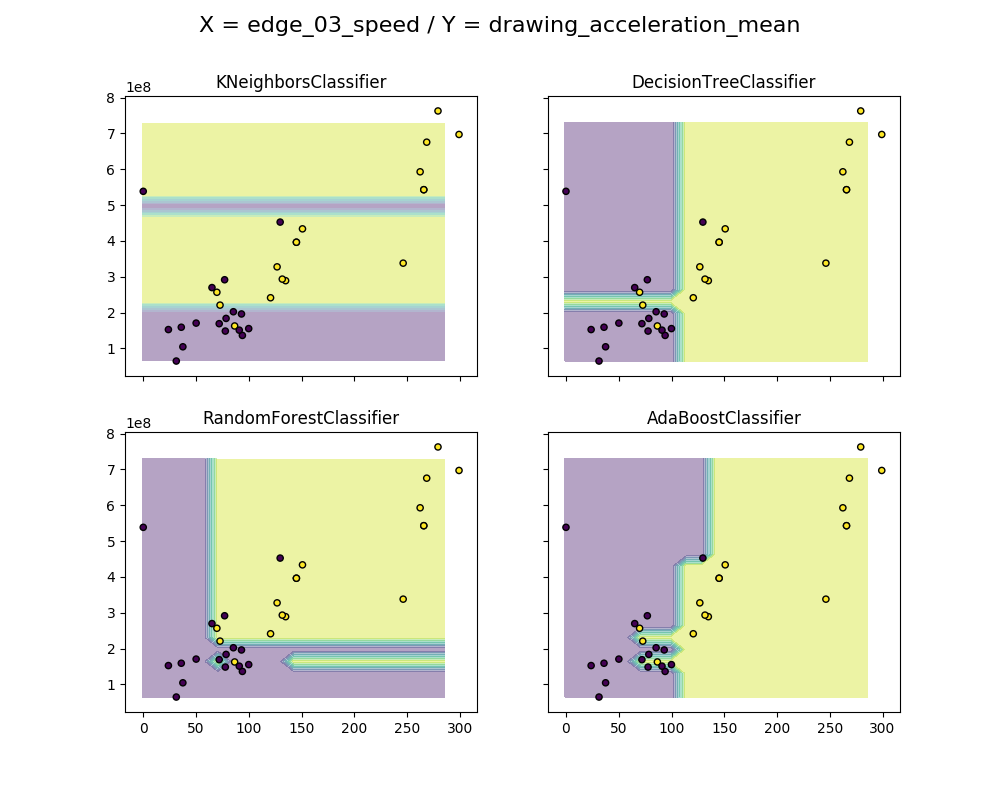
\includegraphics[width=0.85\textwidth, trim=0cm 1.5cm 0cm 0cm]
        {images/classifier/003}
    \caption{Decision Boundaries for PD Classifiers: $x$-axis --- linear speed of third edge of the drawing, $y$-axis --- average acceleration of the drawing. Healthy controls \textit{HC} instances are marked with \textit{yellow} dots.}
    
    \label{classifier2}
\end{figure}

\begin{figure}[htb]
  \centering
    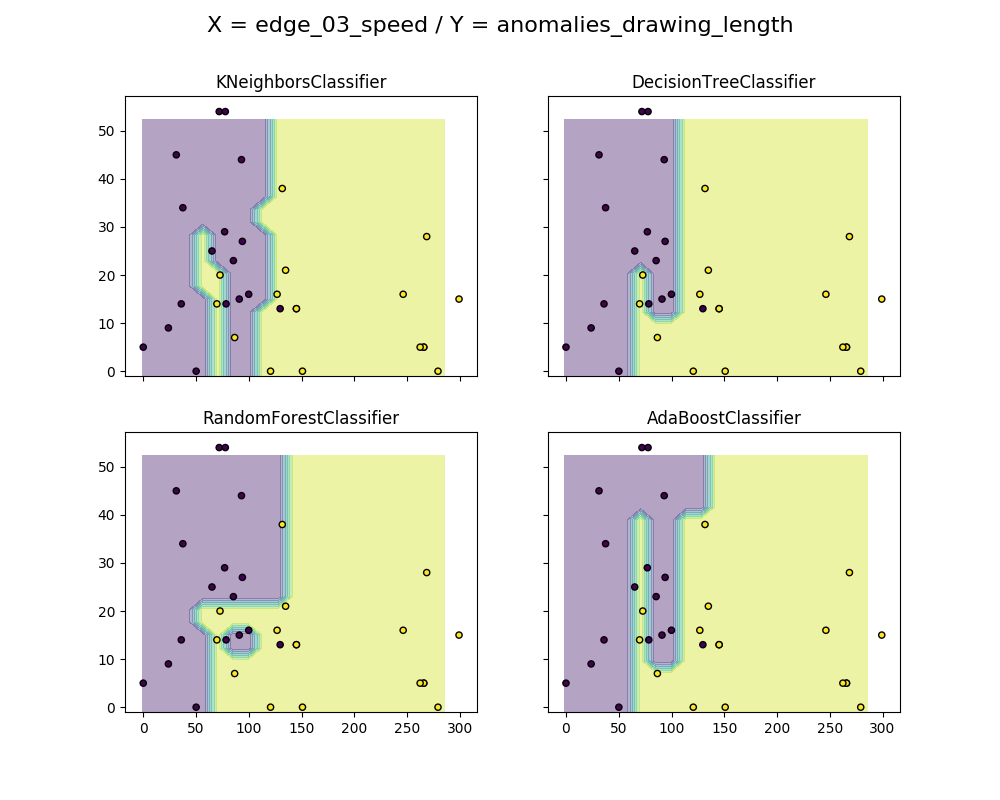
\includegraphics[width=0.85\textwidth, trim=0cm 1.5cm 0cm 0cm]
        {images/classifier/002}
    \caption{Decision Boundaries for PD Classifiers: $x$-axis --- linear speed of third edge of the drawing, $y$-axis --- number of length anomalies in the drawing. Healthy controls \textit{HC} instances are marked with \textit{yellow} dots.}
    
    \label{classifier3}
\end{figure}

\begin{figure}[htb]
  \centering
    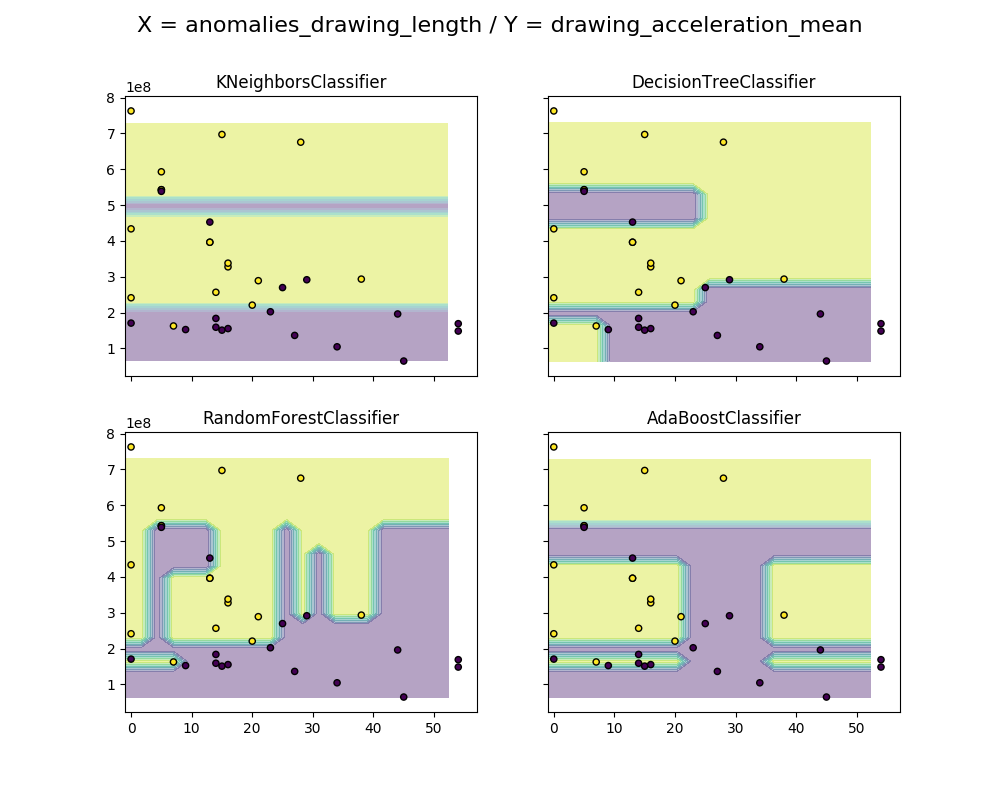
\includegraphics[width=0.85\textwidth, trim=0cm 1.5cm 0cm 0cm]
        {images/classifier/001}
    \caption{Decision Boundaries for PD Classifiers: $x$-axis --- number of length anomalies in the drawing, $y$-axis --- average acceleration of the drawing. Healthy controls \textit{HC} instances are marked with \textit{yellow} dots.}
    \label{classifier4}
\end{figure}

\begin{figure}[htb]
  \centering
    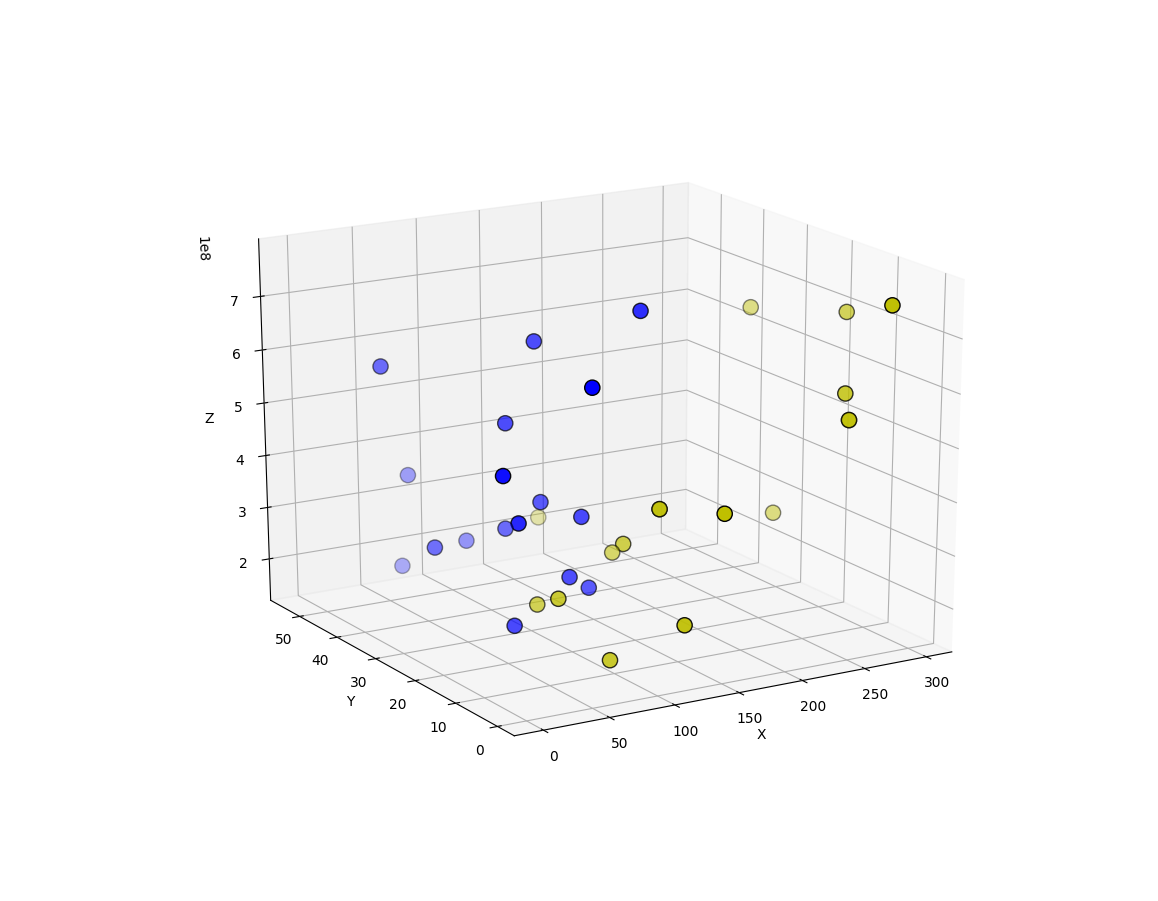
\includegraphics[width=1.0\textwidth, trim=2cm 2.5cm 2cm 3cm, clip=true]
        {images/classifier/004}
    \caption{Dataset of subjects (\textit{HC} --- \textit{yellow}, PD --- \textit{blue}) in 3D feature-space: 
    $X$-axis --- linear speed of third edge of the drawing,
    $Y$-axis --- number of length anomalies in the drawing, 
    $Z$-axis --- average acceleration of the drawing.}
    \label{3d}
\end{figure}